\documentclass[12pt,a4paper]{article}
\usepackage[utf8]{inputenc}
\usepackage[ngerman]{babel}
\usepackage{graphicx}
\usepackage{booktabs} % Für Tabellen
\usepackage{caption}
\usepackage{amsmath}
\usepackage{enumitem} % Paket für bessere Nummerierung
\usepackage{csquotes} 


\usepackage{xcolor}
\usepackage{listings}
 
 

\usepackage{tikz}
\usetikzlibrary{positioning}
\tikzstyle{block} = [rectangle, draw, fill=blue!20, text width=6em, text centered, rounded corners, minimum height=4em]
\tikzstyle{arrow} = [thick,-,>=stealth]


\usepackage{tikz}
\usepackage{hyperref} % Hinzugefügte Option

\usepackage[backend=biber, style=numeric]{biblatex}
\addbibresource{references.bib}
\begin{document}
	
		
		% Titelseite
		\begin{titlepage}
			\begin{center}
				\vspace*{1cm}
				\Huge
				Sprache, Spracheingabe, Text \& Übersetzung mit Google Cloud APIs
				
				
				\vspace{1.5cm}
				\LARGE
				M.Sc. Onur Yilmaz
				
				\vspace{1.5cm}
				\Large
				Angewandte Künstliche Intelligenz
				
				\vfill
				
				Schriftliche Ausarbeitung - Cloud Computing
				\vspace{0.5cm}
				\large
				Fachhochschule Südwestfalen
				\vspace{0.8cm}
				\Large
				\\
				Gutachter: Prof. Dr. Giefers
				\\
				\vspace{0.5cm}
				\large		
				\today
			\end{center}
		\end{titlepage}

\thispagestyle{empty}
\tableofcontents

\newpage
\section*{Einleitung}
In dieser Arbeit werden Technologien und Anwendungen aus dem Bereich der Sprach- und Textverarbeitung beleuchtet, die auf Google Cloud-Diensten aufbauen. Hierzu gehören die \textit{Cloud Speech API}, die \textit{Cloud Translation API}, die \textit{Natural Language API} und die \textit{Text-to-Speech API} \cite{googlecloudskills2023}.
\\ \\
Im ersten Abschnitt, der sich auf \cite{giefers2023cloud} bezieht, wird eine kurze Einführung in die Konzepte des Cloud Computings sowie der API-Integration im Zusammenhang mit NLP-Technologien gegeben, sowie die Interaktion mit der Google Cloud API erläutert.
\\ \\
Der Abschnitt \textit{Spracherkennung und -transkription} fokussiert sich auf die \textit{Cloud Speech API}, die die Transkription von Audio in Text ermöglicht, und die Methoden zur Messung und Verbesserung der Sprachgenauigkeit.
\\ \\
In der \textit{Sprachübersetzung} wird die \textit{Cloud Translation API} behandelt, die den Prozess der Übersetzung von Texten in verschiedene Sprachen ermöglicht.
\\ \\
Der Bereich \textit{Textanalyse} befasst sich mit der \textit{Natural Language API}, die Techniken zur Klassifizierung von Text in Kategorien und zur Analyse von Entitäten und Sentiments bietet.
\\ \\
Im Abschnitt \textit{Sprachsynthese} wird die \textit{Text-to-Speech API} vorgestellt, die die Erzeugung synthetischer Sprache ermöglicht.
\\ \\
Die Arbeit dient nicht nur als theoretischer Überblick, sondern bietet auch praktische Einblicke und Anleitungen zur Verwendung dieser Tools. Dabei werden unterschiedliche Schwierigkeitsgrade und Themenbereiche abgedeckt, um einen umfassenden Einblick in die Möglichkeiten der Sprach- und Textverarbeitung mit Google Cloud zu bieten.

	
\newpage

\section{Cloud Computing und NLP-Technologien}

\subsection{Cloud Computing im Kontext von NLP}
Cloud Computing bezeichnet die Bereitstellung von IT-Ressourcen wie Rechenleistung, Speicherplatz und Anwendungen über das Internet. Anstatt Ressourcen physisch vor Ort zu haben, ermöglicht Cloud Computing den Zugriff auf diese Ressourcen in großen Datenzentren. Dies bietet Unternehmen und Einzelpersonen Flexibilität, Skalierbarkeit und oft Kosteneffizienz. Im Kontext der natürlichen Sprachverarbeitung (NLP) revolutioniert Cloud Computing die Verarbeitung, Analyse und Interpretation großer Mengen von Sprachdaten. Es ermöglicht den Zugriff auf leistungsstarke und skalierbare Ressourcen, die NLP-Projekte effizient und effektiv durchführen.
\subsection{APIs und ihre Rolle im NLP}
Wenn man über Cloud spricht, ist eine der Hauptinteraktionen die Verwendung von APIs. 
\\ \\
Eine \textbf{\textit{API (Application Programming Interface)}} dient als Schnittstelle, die es Entwicklern ermöglicht, bestimmte Funktionen eines Programms oder einer Plattform zu nutzen, ohne sich mit den internen Details auseinandersetzen zu müssen. 
\\ \\
Das Aufrufen einer API, oft als \enquote{API-Anfrage} (\textit{im engl. request})  bezeichnet und ist der Prozess, bei dem ein Programm oder eine Anwendung eine Anforderung an einen Server sendet und eine Antwort zurückerhält.

\ \\ \\
\begin{tikzpicture}
	% Anwendung
	\node[draw,rectangle,fill=blue!20,minimum width=3cm,minimum height=2cm] (app) {Anwendung};
	% API-Server
	\node[draw,rectangle,fill=red!20,minimum width=3cm,minimum height=2cm, right=5cm of app] (api) {API-Server};
	
	% Pfeile für Anfrage und Antwort
	\draw[->, thick] (app.east) -- node[above]{Anfrage} (api.west);
	\draw[->, thick] (api.west) -- node[below]{Antwort} (app.east);
\end{tikzpicture}
\ \\ \\
Ein Großteil der modernen APIs, insbesondere im Cloud-Bereich, basiert auf dem Prinzip von REST (Representational State Transfer).\\ \\
\textit{\textbf{RESTful APIs}} nutzen Standard-HTTP-Methoden und bieten einen einheitlichen und vorhersehbaren Mechanismus, um mit dem Server zu interagieren. Dies erleichtert die Integration in Anwendungen und ermöglicht eine breitere Kompatibilität zwischen verschiedenen Systemen.
\\ \\
Im Kontext von NLP und Cloud Computing bieten RESTful APIs eine schnelle, zuverlässige und sichere Möglichkeit, auf leistungsstarke NLP-Modelle und -Dienste zuzugreifen. Sie ermöglichen es Entwicklern, Daten in Echtzeit zu verarbeiten und sofortige Analysen oder Antworten zu erhalten.
Zum Beispiel Textdaten zu senden und als Antwort eine Analyse oder Übersetzung dieses Textes zu erhalten, wäre eine beliebte und heutzutage häufig gebrauchte Anwendung ist. \\
\begin{center}
	\begin{tikzpicture}
		\node[draw, rectangle, fill=blue!20, minimum width=1cm, minimum height=1cm] (app) {NLP-Anwendung};
		\node[draw, rectangle, fill=red!20, minimum width=1.5cm, minimum height=1.5cm, right=of app, xshift=2cm] (api) {API};
		\node[draw, rectangle, fill=green!20, minimum width=1cm, minimum height=1cm, right=of api, xshift=2cm] (server) {NLP-Modell};
		
		\draw[->] (app) -- (api) node[midway, above] {Texteingabe};
		\draw[->] (api) -- (server) node[midway, above] {Verarbeitung};
		\draw[->] (server) -- (api) node[midway, below] {Antwort};
		\draw[->] (api) -- (app) node[midway, below] {Analyse};
	\end{tikzpicture}
\end{center}
\subsection{Interaktion mit der Google Cloud API}
Die Google Cloud Plattform bietet eine Vielzahl von RESTful APIs, die speziell für NLP-Aufgaben konzipiert sind. Diese APIs profitieren von der leistungsstarken Infrastruktur von Google, welche es Entwicklern ermöglicht, auf fortschrittliche NLP-Funktionen zuzugreifen. Für den Zugriff auf die Google Cloud APIs ist eine Authentifizierung erforderlich, die häufig über \textbf{\textit{API-Keys}} erfolgt. Sobald die Authentifizierung erfolgreich ist, können Entwickler Daten senden, diese verarbeiten lassen und die Ergebnisse für ihre spezifischen Anwendungen oder Analysen abrufen.


%%%%%%%%%%%%%%%%%%%%%%%%%%%%%%%%%%%%%%%%%%%%%%%%%%%%%%%%%%%%%%%%%%%%%%%%%%%%%%%%%%%%%%%%%%%%%%
\newpage

\section{Spracherkennung und Transkription}
In diesem Abschnitt behandeln wir den Prozess der Spracherkennung und Texttranskription (siehe \cite{towards}), einschließlich der Nutzung der Google Cloud Speech API zur Konvertierung von gesprochener Sprache in Textform \cite{speechtotext2023}. Um hochwertige Transkriptionen zu erhalten, werden wir außerdem auf die Messung und Verbesserung der Genauigkeit bei der Spracherkennung eingehen. Hierbei stützen wir uns auf \cite{speechaccuracy2023}.
\subsection{Sprache-zu-Text-Prozess}
Die Automatische Spracherkennung (ASR), auch als maschinelles Transkribieren oder Sprache-zu-Text bezeichnet, nutzt fortschrittliche Methoden des maschinellen Lernens, um gesprochene Audioinhalte in geschriebenen Text zu verwandeln. Die Einsatzmöglichkeiten sind äußerst vielfältig und reichen von der Erstellung von Untertiteln über die Unterstützung virtueller Assistenten bis hin zur Realisierung interaktiver Sprachsysteme.
\\ \\
Der Prozess beginnt mit der Erfassung der gesprochenen Sprache, sei es mittels eines Mikrofons oder anderer Audioeingaben. Die aufgenommenen Audiosignale werden in diskrete Zeitfenster von typischerweise 10 bis 25 ms unterteilt, die als Sprachrahmen bezeichnet werden. Diese Sprachrahmen fungieren als die elementaren Bausteine, auf denen das ASR-System operiert.
\\ \\
In der nächsten Phase erfolgt die akustische Modellierung. Dieser Schritt umfasst die Analyse der individuellen Sprachrahmen mit dem Ziel, die darin enthaltenen zugrundeliegenden Klänge, als \textit{Phoneme} bekannt, zu identifizieren. Phoneme sind die kleinsten distinkten sprachlichen Einheiten, die den Bausteinen der Wörter zugrunde liegen. Das akustische Modell nutzt ein Trainingskorpus, um auf akkurate Weise die Charakteristiken der Klangmuster in den Audiosignalen zu erfassen und diesen Mustern die entsprechenden Phoneme zuzuordnen.
\\ \\
In der Anschlussphase durchläuft die erkannte Phonemsequenz das Sprachmodell. Das Sprachmodell nutzt die geordnete Abfolge der Phoneme, um kohärente Wörter und Sätze zu generieren, die den erkannten Lauten entsprechen. Dieser Schritt stellt einen essentiellen Bestandteil dar, um die gesprochene Äußerung in einen verständlichen und grammatikalisch korrekten schriftlichen Ausdruck zu transformieren.
\\ \\
Am Ende dieses Prozesses präsentiert das ASR-System den transkribierten Text als Endergebnis. Hier sieht man eine vereinfachte Darstellung dieses Modelles:
\begin{figure}[h!]
	\centering
	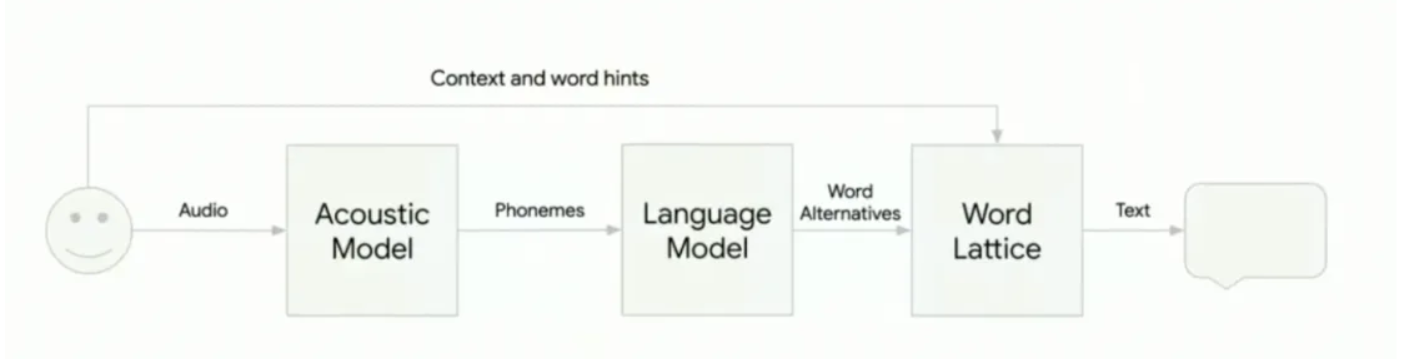
\includegraphics[width=1\linewidth]{../images/STT}
	\caption{\textit{Speech-to-Text} - Prozess}
	\label{fig:stt}
\end{figure}
\subsubsection{Mathematischer Hintergrund}
\subsubsection{Messung und Verbesserung der Sprachgenauigkeit}
Die Genauigkeit der Spracherkennung kann auf verschiedene Arten gemessen werden. Je nach Bedarf können mehrere Metriken verwendet werden. Der branchenübliche Vergleich erfolgt jedoch oft mithilfe des Wortfehlerquotienten (Word Error Rate, WER). Die Wortfehlerquote misst den Prozentsatz falscher Transkriptionen im gesamten Satz. Eine niedrigere WER bedeutet daher, dass das System genauer ist.
\\ \\
In Bezug auf die Genauigkeit der ASR sehen Sie möglicherweise auch den Begriff \textit{Ground Truth}. Ground Truth bezieht sich auf die zu 100\% genaue (in der Regel menschliche) Transkription, mit der Sie die Genauigkeit vergleichen.
\\ \\
\underline{\textbf{Wortfehlerquote (WER):}}
\\ \\
Die Wortfehlerquote setzt sich aus drei Arten von Transkriptionsfehlern zusammen, die auftreten können:

\begin{itemize}
	\item Einfügefehler (I): Wörter, die in der Transkription vorhanden sind, jedoch nicht in der Ground-Truth-Transkription.
	\item Substitutionsfehler (S): Wörter, die sowohl in der Transkription als auch in der Ground Truth vorhanden sind, aber nicht korrekt transkribiert wurden.
	\item Löschungsfehler (D): Wörter, die in der Transkription fehlen, jedoch in der Ground-Truth-Transkription vorhanden sind.
\end{itemize}
\ \\
Die Formel für die WER lautet: 
\[ \text{WER} = \frac{S + D + I}{N} \]
\\
Die Anzahl der Fehler jeder der drei Arten wird summiert und durch die Gesamtzahl der Wörter (N) in der Ground-Truth-Transkription geteilt, um die Wortfehlerquote (WER) zu ermitteln. Dies bedeutet, dass die WER in Situationen mit sehr geringer Genauigkeit größer als 100\% sein kann.


\subsection{Cloud Speech API}
\subsubsection{Erstellen eines API-Keys}
Wir beschreiben nun die Schritte, um einen API-Schlüssel zu erstellen und der uns über der SSH bereitgestellten Linux-Instanz verbinden zu können.
\\ \\
Um die Cloud Speech API mithilfe von \texttt{curl} anzusprechen, benötigen wir einen API-Schlüssel, der in der Anfrage-URL übergeben wird. Hier sind die Schritte zur Erstellung eines API-Schlüssels:
\begin{enumerate}
	\item Wir klicken im Navigationsmenü zu \enquote{APIs \& Services $>$ Anmeldedaten}.
	
	\item Klicken anschließend auf \enquote{Zugangsdaten erstellen (\textit{im engl. Credentials})} und wählen \enquote{API-KEY} aus.
	
	\item Bewahren die erstellte API-Schlüssel sicher auf, da wir diesen später in unserer Entwicklungsumgebung als Variable verwenden werden.
	
	\item Wir klicken anschließend auf \enquote{Schließen}.
\end{enumerate}
\begin{figure}[h!]
	\centering
	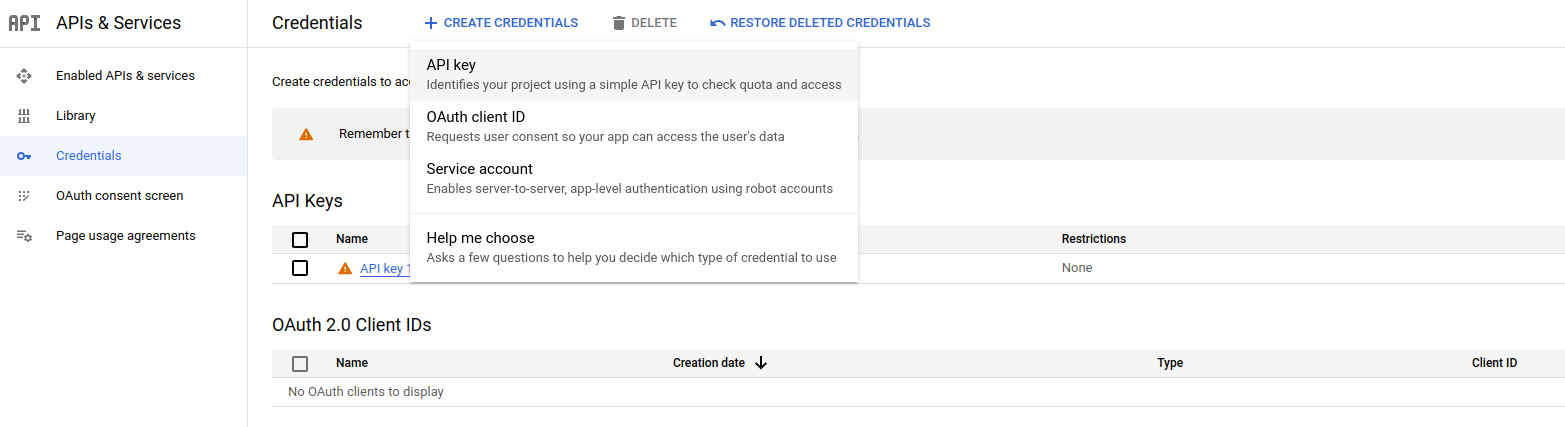
\includegraphics[width=1\linewidth]{../images/GCP_CREATE_API}
	\caption{Erstellen eines API-KEYs in GCP}
	\label{fig:gcpcreateapi}
\end{figure}
\ \\
Um die nächsten Schritte auszuführen, verbinden wir uns mit der Ihnen bereitgestellten Linux-Instanz über SSH:
\begin{enumerate}
	\item Navigieren im Navigationsmenü zu \enquote{Compute Engine $>$ VM-Instanzen}.
	
	\item Suchen die Linux-Instanz VM in der Liste der VM-Instanzen. 
	
	\item Klicken rechts neben dem Namen der Linux-Instanz auf \enquote{SSH}, um eine interaktive Shell zu öffnen. Diese Shell verwenden wir, um die nächsten Schritte auszuführen.

\begin{figure}[h!]
	\centering
	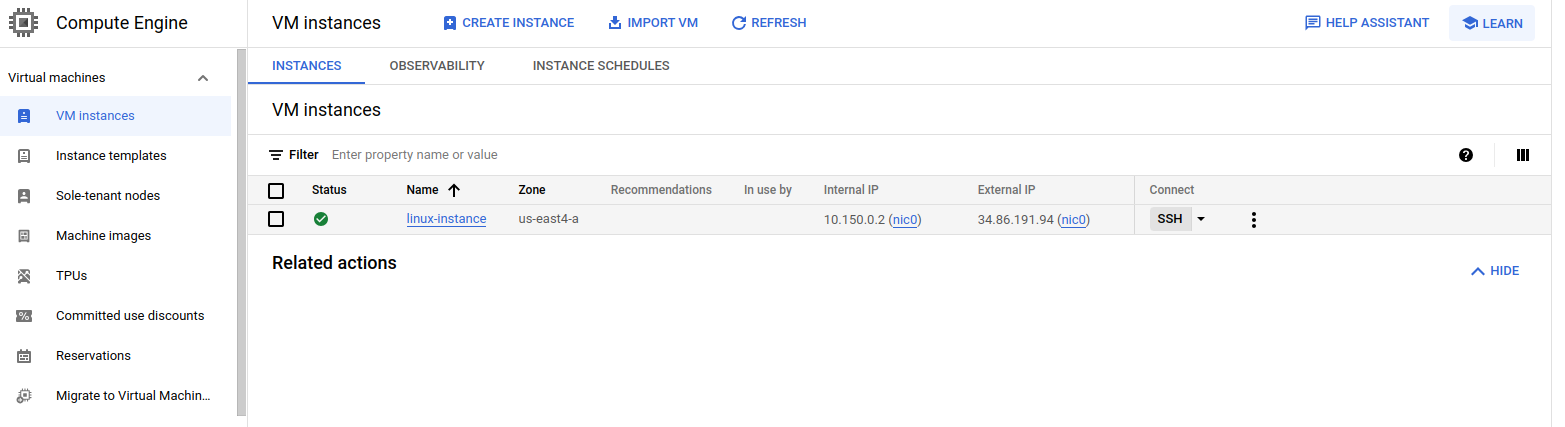
\includegraphics[width=0.9\linewidth]{../images/VM_Instances}
	\caption{VM Instanz}
	\label{fig:vminstances}
\end{figure}

	\item In der geöffneten SSH-Shell führen wir den folgenden Befehl aus und ersetzen den KEY durch den von uns zuvor erstellten API-Schlüssel:

\begin{figure}[h!]
	\centering
	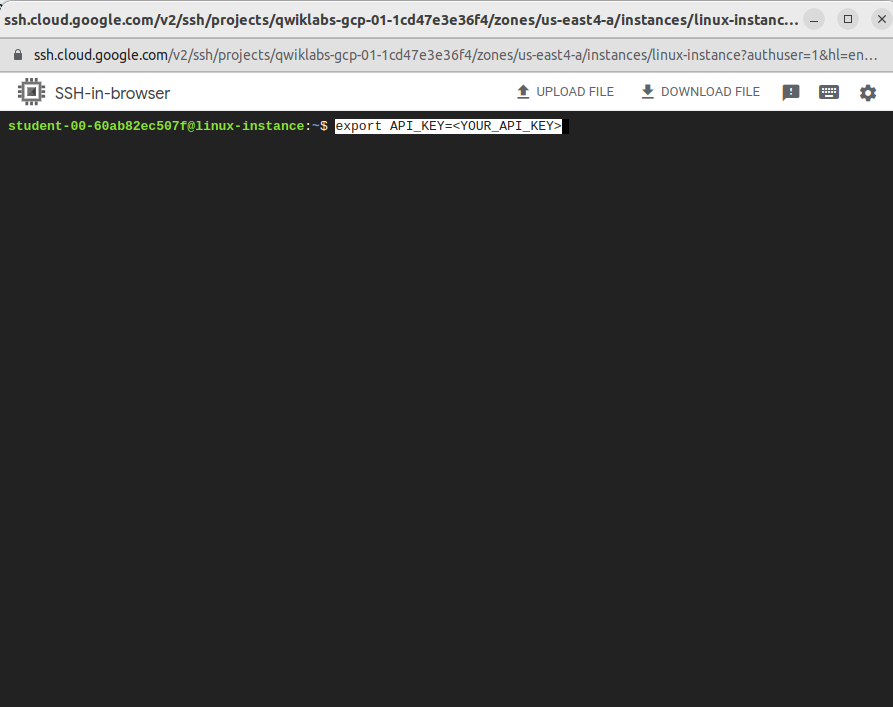
\includegraphics[width=0.7\linewidth]{../images/SSH}
	\label{fig:ssh}
\end{figure}
\end{enumerate}
\ \\ \\
Der nächste Schritt ist die Verwendung von \texttt{curl}, um eine Anfrage an die Cloud Speech API zu senden und die gewünschten Transkriptionen zu erhalten. 
\subsubsection{Erstellen der API-Anfrage}
\begin{enumerate}
\item Wir erstellen unsere Anfrage an die API in einer \texttt{request.json}-Datei. Die Datei \texttt{request.json} kann wie folgt erstellt werden:
\begin{center}
\verb|touch request.json|
\end{center}
\item Anschließend öffnen wir die Datei mit unserem bevorzugten Editor (nano, vim, emacs) und fügen Folgendes zu unserer \texttt{request.json}-Datei hinzu:
\begin{figure}[h!]
\centering
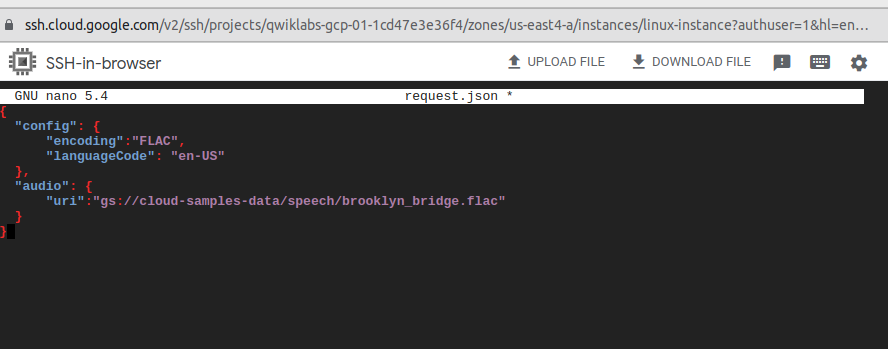
\includegraphics[width=0.9\linewidth]{../images/request_json}
\label{fig:requestjson}
\end{figure}
\ \\
Hier obiger Code noch einmal übersichtlich dargestellt:
\begin{verbatim}
	{
		"config": {
			"encoding":"FLAC",
			"languageCode": "en-US"
		},
	
		"audio": {
			"uri":"gs://cloud-samples-data/speech/brooklyn_bridge.flac"
		}
	}
\end{verbatim}
Nachdem wir uns den obigen JSON-Code erstellt haben, werfen wir einen Blick über die einzelnen Bestandteile
\begin{itemize}
	\item \enquote{config}: Dies ist ein Objekt, das Konfigurationseinstellungen enthält.
	
	\item \enquote{encoding}: \enquote{FLAC}: Dies legt das Encoding (Datenformat) für den Audiodatenstrom fest. In diesem Fall wird das FLAC-Format verwendet, das ein verlustfreies Audioformat ist.
	
	\item \enquote{languageCode}: \enquote{en-US}: Dies gibt den Sprachcode an. Hier ist es \enquote{en-US}, was auf US-Englisch hinweist.
	
	\item \enquote{audio}: Dies ist ebenfalls ein Objekt, das Informationen über die Audiodaten enthält.
	
	\item \enquote{uri}: \enquote{gs://cloud-samples-data/speech/brooklyn\_bridge.flac}: Dies ist die URI (Uniform Resource Identifier) oder der Pfad zum Audiofile. In diesem Fall handelt es sich um eine Audioaufnahme der Brooklyn Bridge im FLAC-Format, die in der Google Cloud Storage (gs) gespeichert ist.
\end{itemize}

\end{enumerate}
\subsubsection{Aufrufen der API}



%%%%%%%%%%%%%%%%%%%%%%%%%%%%%%%%%%%%%%%%%%%%%%%%%%%%%%%%%%%%%%%%%%%%%%%%%%%%%%%%%%%%%%%%%%%%%%

\newpage
\section{Sprachübersetzung}

In diesem Abschnitt wird die Erkennung und Übersetzung von Texten behandelt, um verschiedene Sprachen zu übersetzen. Hierbei wird auf die Möglichkeiten der Cloud Translation API von Google Cloud eingegangen \cite{cloudtranslation2023}.
\subsection{Erkennung und Übersetzung von Texten}
\subsection{Cloud Translation API}
\newpage

\section{Textanalyse}
In diesem Abschnitts steht die Klassifizierung von Texten in verschiedene Kategorien im Vordergrund. Dabei wird erläutert, wie die Natural Language API von Google Cloud eingesetzt werden kann, um Texte einer gründlichen Analyse zu unterziehen und sie in entsprechende Kategorien einzuordnen \cite{classtext2023}. Doch die Möglichkeiten gehen noch weiter. 
\\ \\
Durch die Entitäten- und Sentimentanalyse gewinnen wir tiefere Einblicke in die Texte. Diese Analysetechniken ermöglichen es, bedeutende Entitäten innerhalb des Textes zu identifizieren sowie die generelle Stimmung und emotionale Tonalität des Textinhalts zu erfassen. Dieser Abschnitt beleuchtet die vielfältigen Anwendungsgebiete der Natural Language API von Google Cloud auf diesem Gebiet \cite{entitysentiment2023}.
\subsection{Klassifizierung von Text in Kategorien}
\subsection{Entitäten- und Sentimentanalyse}
\subsection{Natural Language API}


\newpage

\section{Sprachsynthese}
Die Erzeugung synthetischer Sprache mittels Text-to-Speech-Technologie wird in diesem Abschnitt behandelt. Dabei wird beschrieben, wie die Natural Language API von Google Cloud genutzt werden kann, um aus Texten künstliche Sprachausgaben zu erzeugen \cite{texttospeech2023}.
\subsection{Erzeugung synthetischer Sprache}
\subsection{Natural Language API}



\newpage
\thispagestyle{empty}
\printbibliography

\end{document}
